\section{Metodologia}
	
	O processo metodológico escolhido para desenvolvimento do R2-PI2 é baseado em uma metodologia ágil, mais especificamente, no \textit{Scrum}. Dessa forma, o processo como um todo será dividido \textit{releases}, contemplando \textit{sprints} de 2 semanas, em média. Antes de definirmos o processo de maneira específica, é necessário apresentar uma visão alto nível do projeto inteiro, destacando os pontos de controle e deixando claras as atividades críticas para o sucesso do projeto.

	Com este objetivo, o processo apresentado na Figura \ref{img:processo_geral} foi modelado, utilizando a ferramenta \textit{Bizagi Modeler}\footnote{http://www.bizagi.com/pt/}.

	\begin{figure}[H]
		\centering
		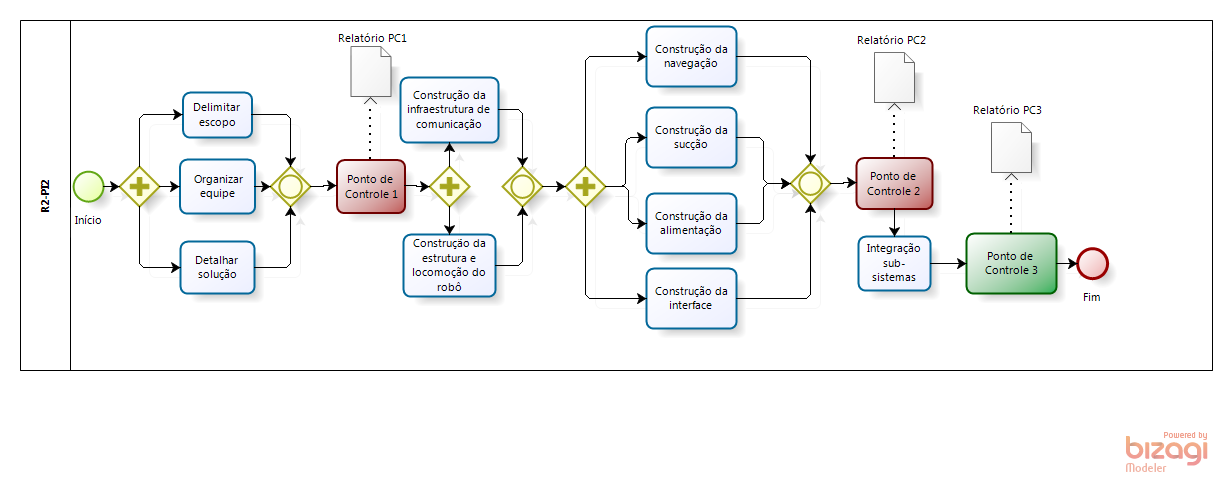
\includegraphics[scale=0.6]{figuras/processo_geral.png}
		\caption{Processo geral de desenvolvimento da solução.}
		\label{img:processo_geral}
	\end{figure}

	As atividades presentes no processo estão descritas abaixo.

	\begin{itemize}
		\item \textbf{Delimitar escopo}:

			Etapa de levantamento dos requisitos, onde é definido tudo que está dentro do projeto, que será implementado, e tudo que está fora, ou seja, que não será implementado.

		\item \textbf{Organizar equipe}:

			Etapa que busca definir uma política de comunicação da equipe, discute e define com todos os integrantes a metodologia e a rotina de trabalho que serão seguidas e define papéis e/ou responsabilidades.


	\end{itemize}

	\subsection{Cronograma} % (fold)
	\label{sub:cronograma}
		Apresentar o cronograma de atividades relacionado ao Scrum, destacando os pontos de controle.
	% subsection cronograma (end)
